% ── IRF ──────────────────────────────────────────────────────────────────────
\begin{frame}{Impulse response functions — uncertainty shocks on IGAE}

\begin{columns}[T]

\begin{column}{0.60\textwidth}
\begin{figure}
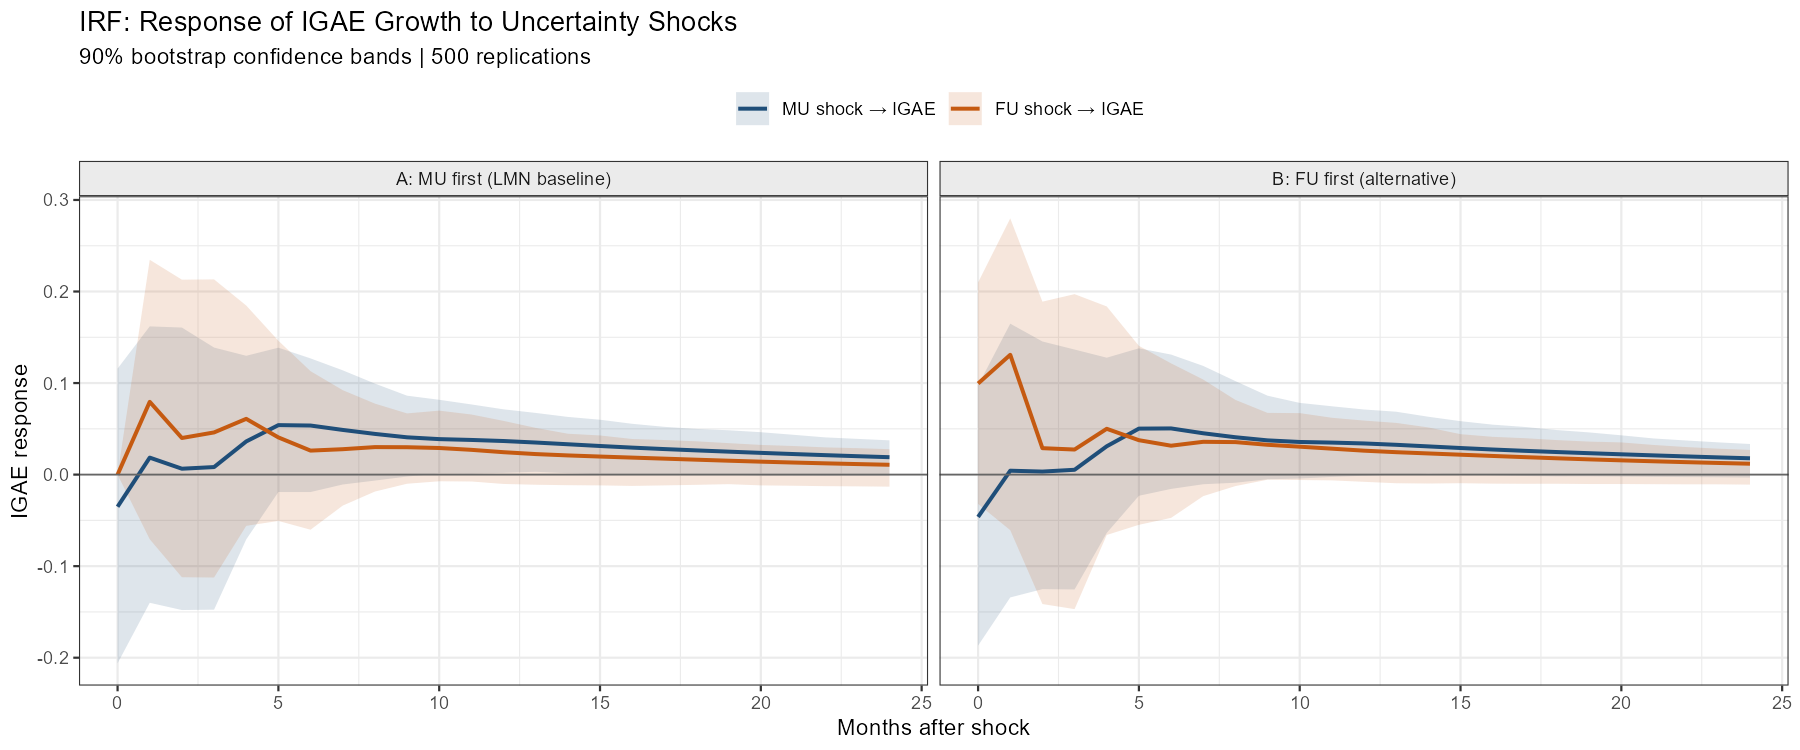
\includegraphics[scale=.45]{../ioae_assesment/outputs/lmn/fig4_irfs.png}
\end{figure}
\end{column}

\begin{column}{0.37\textwidth}
\small
\begin{itemize}
  \item \textbf{MU shock:} IGAE response is negative on impact and mean-reverts by month 6--8. Path is \textbf{stable across orderings} — macro uncertainty identification is robust.

  \vspace{2mm}

  \item \textbf{FU shock (Ordering A, FU last):} response is near zero — the Cholesky restriction prevents a contemporaneous FU$\to$IGAE channel by construction.

  \vspace{2mm}

  \item \textbf{FU shock (Ordering B, FU first):} larger negative impact on IGAE, confirming that FU's effect operates primarily \textbf{within the same month}.

  \vspace{2mm}

  \item 90\% bootstrap bands; both channels are statistically modest — consistent with a small open economy where external demand dominates output fluctuations.
\end{itemize}
\end{column}

\end{columns}
\end{frame}


% ── FEVD ─────────────────────────────────────────────────────────────────────
\begin{frame}{Forecast error variance decomposition — IGAE growth}

\begin{columns}[T]

\begin{column}{0.60\textwidth}
\begin{figure}
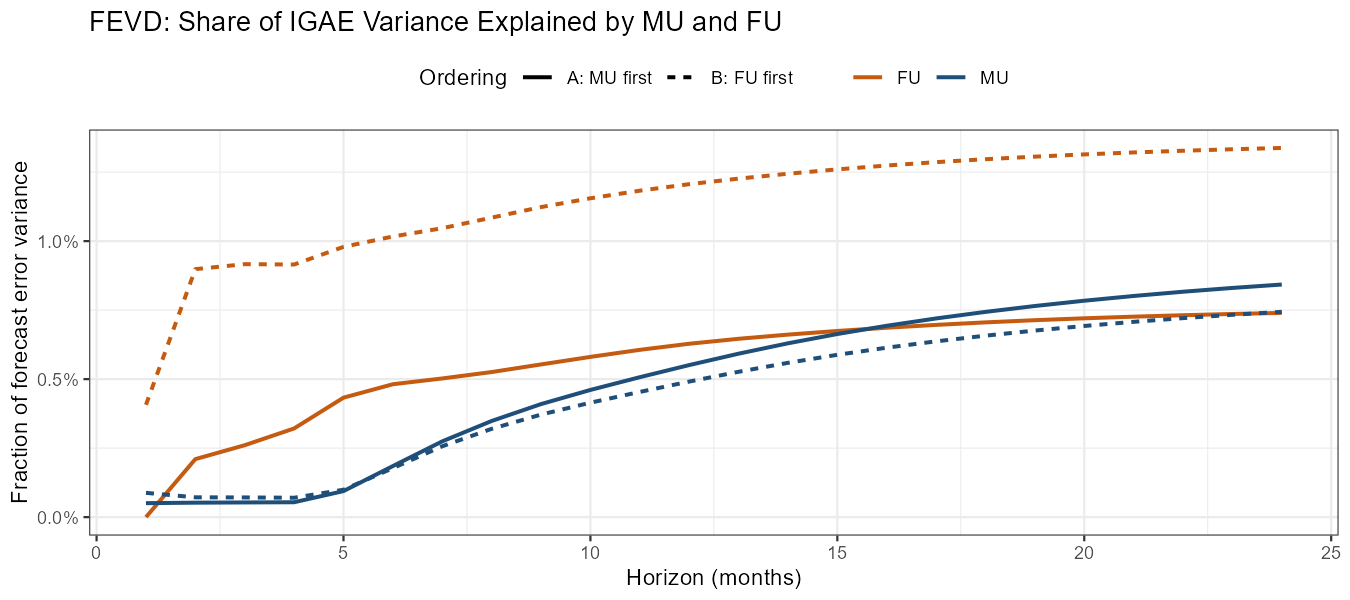
\includegraphics[scale=.50]{../ioae_assesment/outputs/lmn/fig5_fevd.png}
\end{figure}
\end{column}

\begin{column}{0.37\textwidth}
\small
\begin{itemize}
  \item \textbf{IGAE own dynamics dominate} at all horizons (97--99\%), reflecting strong output persistence and the large role of external demand.

  \vspace{2mm}

  \item \textbf{MU contributes $\approx$0.8\%} and is insensitive to ordering — its causal role is identified the same way regardless of where FU sits.

  \vspace{2mm}

  \item \textbf{FU is ordering-sensitive:} 0.3\% when ordered last (no contemporaneous channel) vs.\ 2.3\% when ordered first. The gap is the \textbf{within-month FU effect}.

  \vspace{2mm}

  \item Combined MU+FU share (1--3\%) is small but in line with uncertainty-channel estimates for emerging markets in the literature.
\end{itemize}
\end{column}

\end{columns}
\end{frame}


% ── LP IRF ───────────────────────────────────────────────────────────────────
\begin{frame}{Local projections vs.\ VAR — robustness check}

\begin{columns}[T]

\begin{column}{0.60\textwidth}
\begin{figure}
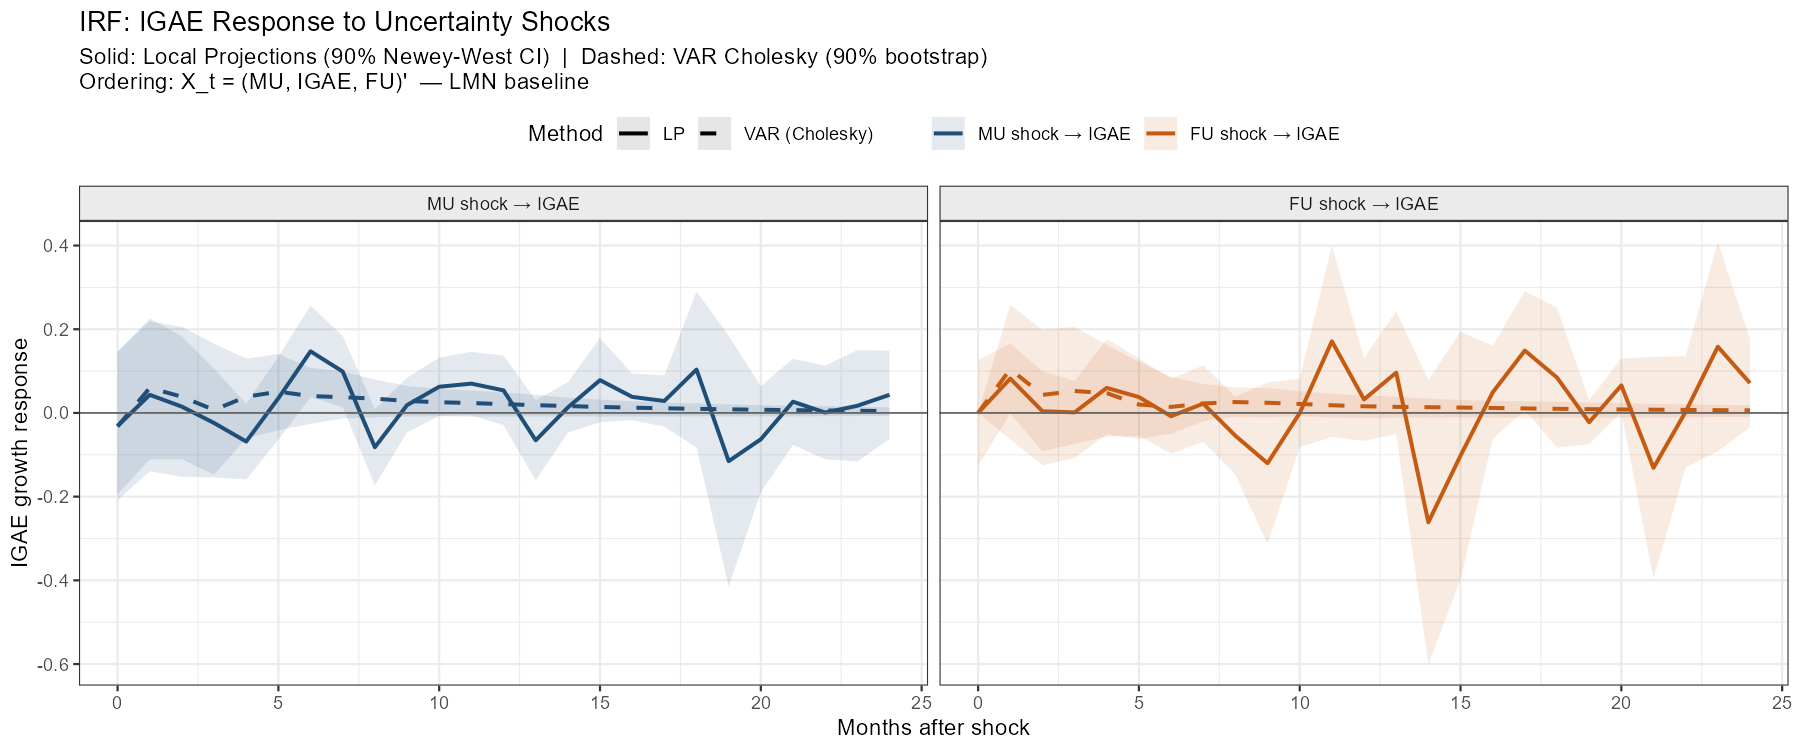
\includegraphics[scale=.45]{../ioae_assesment/outputs/lmn/fig6_lp_irf.png}
\end{figure}
\end{column}

\begin{column}{0.37\textwidth}
\small
\begin{itemize}
  \item \textbf{LP (solid) and VAR (dashed) trace similar paths} — no evidence of mis-specification accumulation in the VAR across horizons.

  \vspace{2mm}

  \item \textbf{LP bands are wider} by construction: Newey-West HAC accounts for the MA($h-1$) serial correlation induced by overlapping projection windows.

  \vspace{2mm}

  \item Zero lies within most confidence bands for both methods — confirming that uncertainty shocks generate \textbf{statistically modest} output responses.

  \vspace{2mm}

  \item Consistency between LP and VAR validates the FEVD decomposition: the VAR's parametric structure is not driving the small uncertainty shares.
\end{itemize}
\end{column}

\end{columns}
\end{frame}
